\begin{table}[h!]
\centering
\caption{Geometric and Internal Core Parameters in the Sangamon Reactors}
\begin{tabular}{ c  c  c }
\hline
Parameter & Sangamon200 \cite{harlan_x-energy_2018}, \cite{harlan_ans_2017} & Sangamon20 \\
\hline
Thermal Power [MW] & 200 & 20 \\
Average Core Temperature [K] & 800 & 800 \\
Enrichment [wt\%] & 15.5\% & 19.75\% \\
Average Core Pressure [MPa] & 5.9 & 5.9 \\
Outer Core Radius [cm] & 216 & 165 \\
Outer Core Height [cm] & 1150 & 330 \\
Reflector Thickness [cm] & 92 & 75 \\
Number of Pebbles & 220,000 & 22,680 \\
Packing Fraction [\%] & 53.0 & 56.0 \\
\hline
\end{tabular}

\label{table:params1}
\end{table}

All neutronics simulations are performed using Serpent2.0 \cite{leppanenjaakko_serpent_2015} .  Pebbles are individually modeled, with locations generated using Serpent2.0's particle dispersal routine (***should I go into more detail on the dispersal routine?***).  Each pebble in the full-core model has the TRISO-filled "fueled-core" homogenized by volume.
\\
\begin{figure}[H]
\centering


\includegraphics[width=0.5\linewidth]{figures/pebble-zones.png}
\caption{Pebble Zones}
\label{fig:pebb-zone1}
\end{figure}


\begin{table}[h!]
\centering

\caption{Pebble Parameters}
\begin{tabular}{ c  c }
\hline
Parameter & Value \\
\hline
Fueled-Center Radius [cm] & 2.5 \\
Graphite Outer Shell Thickness [cm] & 0.5 \\
Total Radius [cm] & 3.0 \\
TRISO Particles per Pebble & 18,000 \\
\hline
\end{tabular}
\label{table:peb-params}
\end{table}


\begin{figure}[H]
\centering

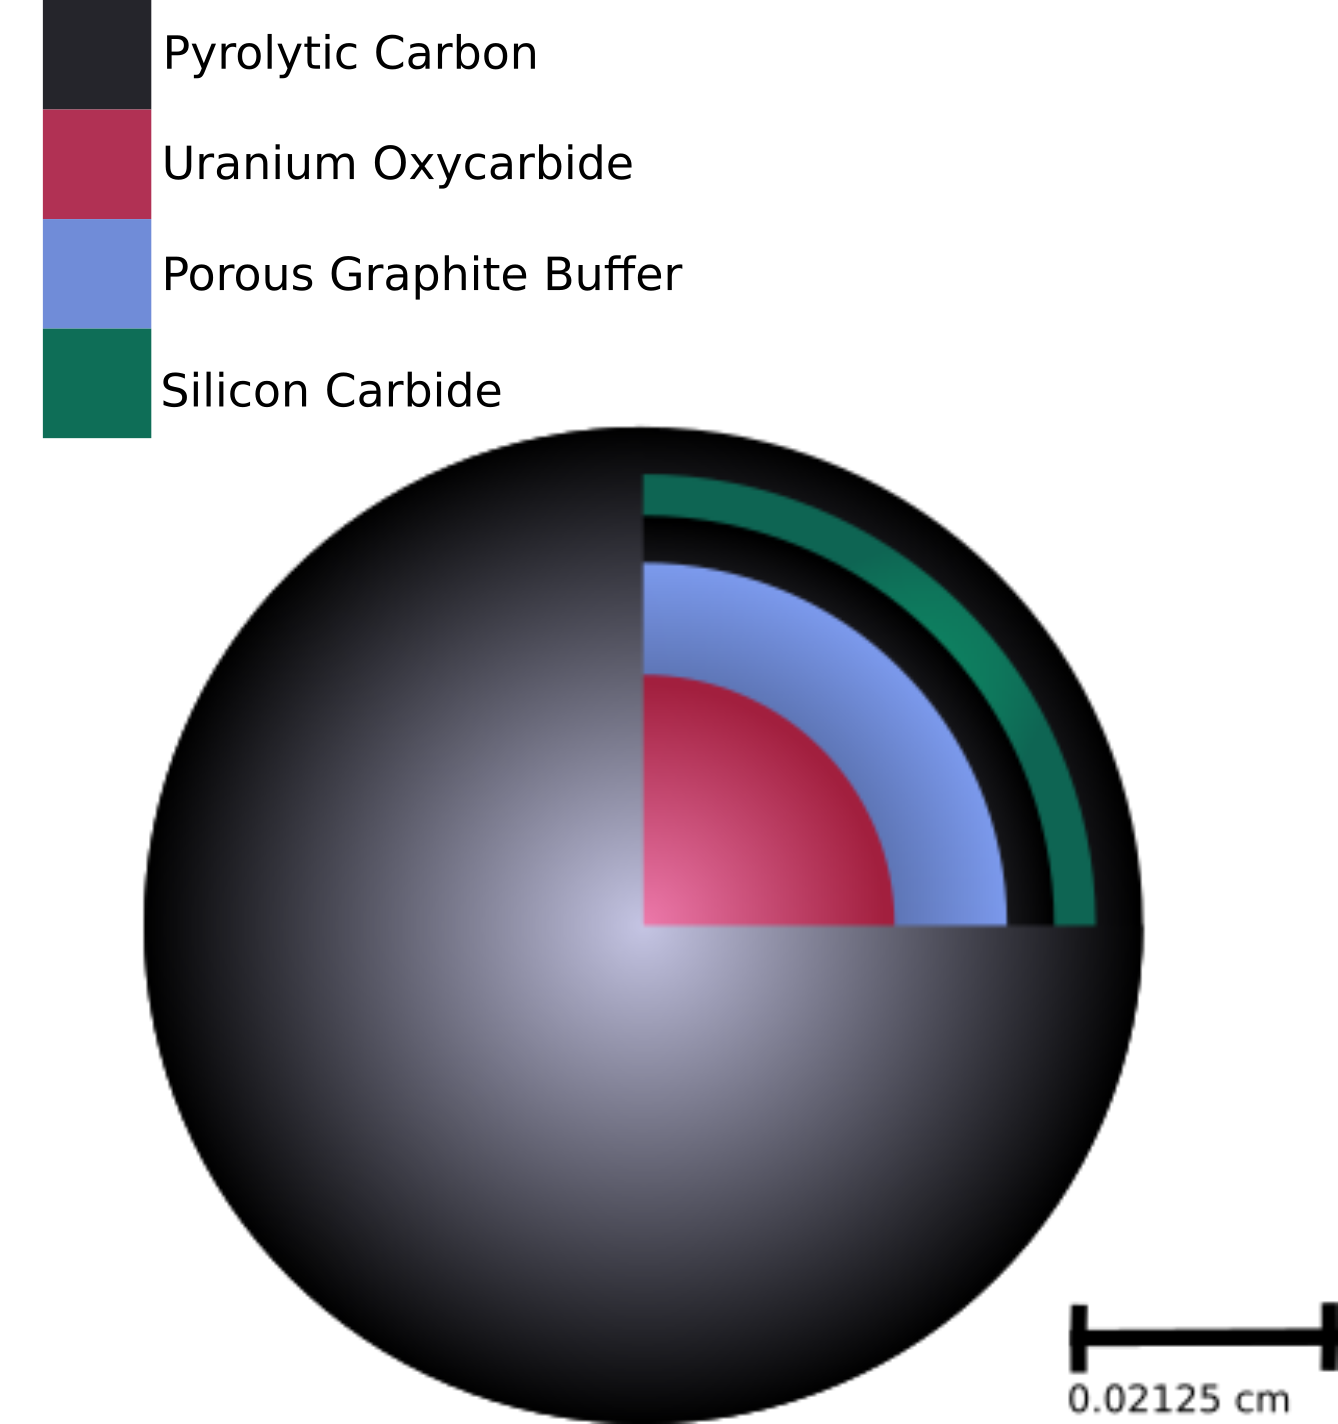
\includegraphics[width=0.5\linewidth]{figures/trisos-r-like-onions.png}
\caption{TRISO Particle Layers}
\label{fig:particle-layer}
\end{figure}

\begin{table}[h!]
\centering

\caption{Particle Parameters Used in Monte Carlo Simulations}
\begin{tabular}{ c  c }
\hline
Parameter & Value [cm] \\
\hline 
Uranium Oxycarbide Kernel Radius & 0.02125 \\
Graphite Layer Thickness & 0.03075 \\
Inner Pyrolytic Carbon Layer Thickness & 0.03475 \\
Silicon Carbide Layer Thickness & 0.03825 \\
Outer Pyrolytic Carbon Layer Thickness & 0.04225 \\
\hline
\end{tabular}
\label{table:particle-params}

\end{table}

\begin{table}[h!]
\centering
\begin{tabular}{ c  c }
\hline
Parameter & Value \\
\hline
Fueled-Center Radius [cm] & 2.5 \\
Graphite Outer Shell Thickness [cm] & 0.5cm \\
Total Radius [cm] & 3.0 \\
TRISO Particles per Pebble & 18,000 \\
\hline
\end{tabular}
\caption{Pebble Parameters}
\label{table:params2}
\end{table}
\begin{table}[h!]
\centering
\begin{tabular}{|| c || c |}
\hline
Parameter & Value \\
\hline \hline
Uranium Oxycarbide Kernel Radius [cm] & 0.02125 \\
Graphite Layer Thickness [cm] & 0.03075 \\
Inner Pyrolytic Carbon Layer Thickness [cm] & 0.03475 \\
Silicon Carbide Layer Thickness [cm] & 0.03825 \\
Outer Pyrolytic Carbon Layer Thickness [cm] & 0.04225 \\
\hline
\end{tabular}
\caption{Particle Parameters}
\label{table:params3}
\end{table}
\\
Fuel isotopic composition aside, the pebbles are identical in both reactor designs.  Both reactors feature a 6-month multi-pass cycle, with each pass through the core taking 6 months.  That is to say, a pebble will go through six 6-month passes before leaving the core.

\section{Sangamon0}
Sangamon0 is a 200 MWth helium cooled reactor.  It is an Xe-100 inspired design, and further informed by previous work on reactors such as the PBMR and NGNP.  Parameters are generally pulled from literature, or made by averaging given values in literature.  For reactor dimensions that are not specified, a rough estimate is approximated by assuming provided figures of a design are to scale, and converting measurements in pixels to cm.

Sangamon0 is still, however, a simplification of previously established designs.  The "cone" formed at the top and bottom of the reactor core is averaged to a flat surface, to create a cylindrical core shape.  The graphite reflector surrounds it, with no barriers between the reflector and helium/pebble-filled active core region.  In effect, the reflector is the "container" for the pebbles.  These are the only parts of the reactor that have been modeled.  It is assumed no control rods are being used.  In addition, the graphite reflector is modeled as solid.

While Sangamon0 is not the focus of this assessment, some neutronics features were determined to aid in Sangamon1's design.  A surface current detector was placed in the reflector, just inside the outer bound of the reflector, as shown in \ref{fig:det-place}.

\begin{figure}[H]
\centering
\resizebox{0.5\textwidth}{!}{%
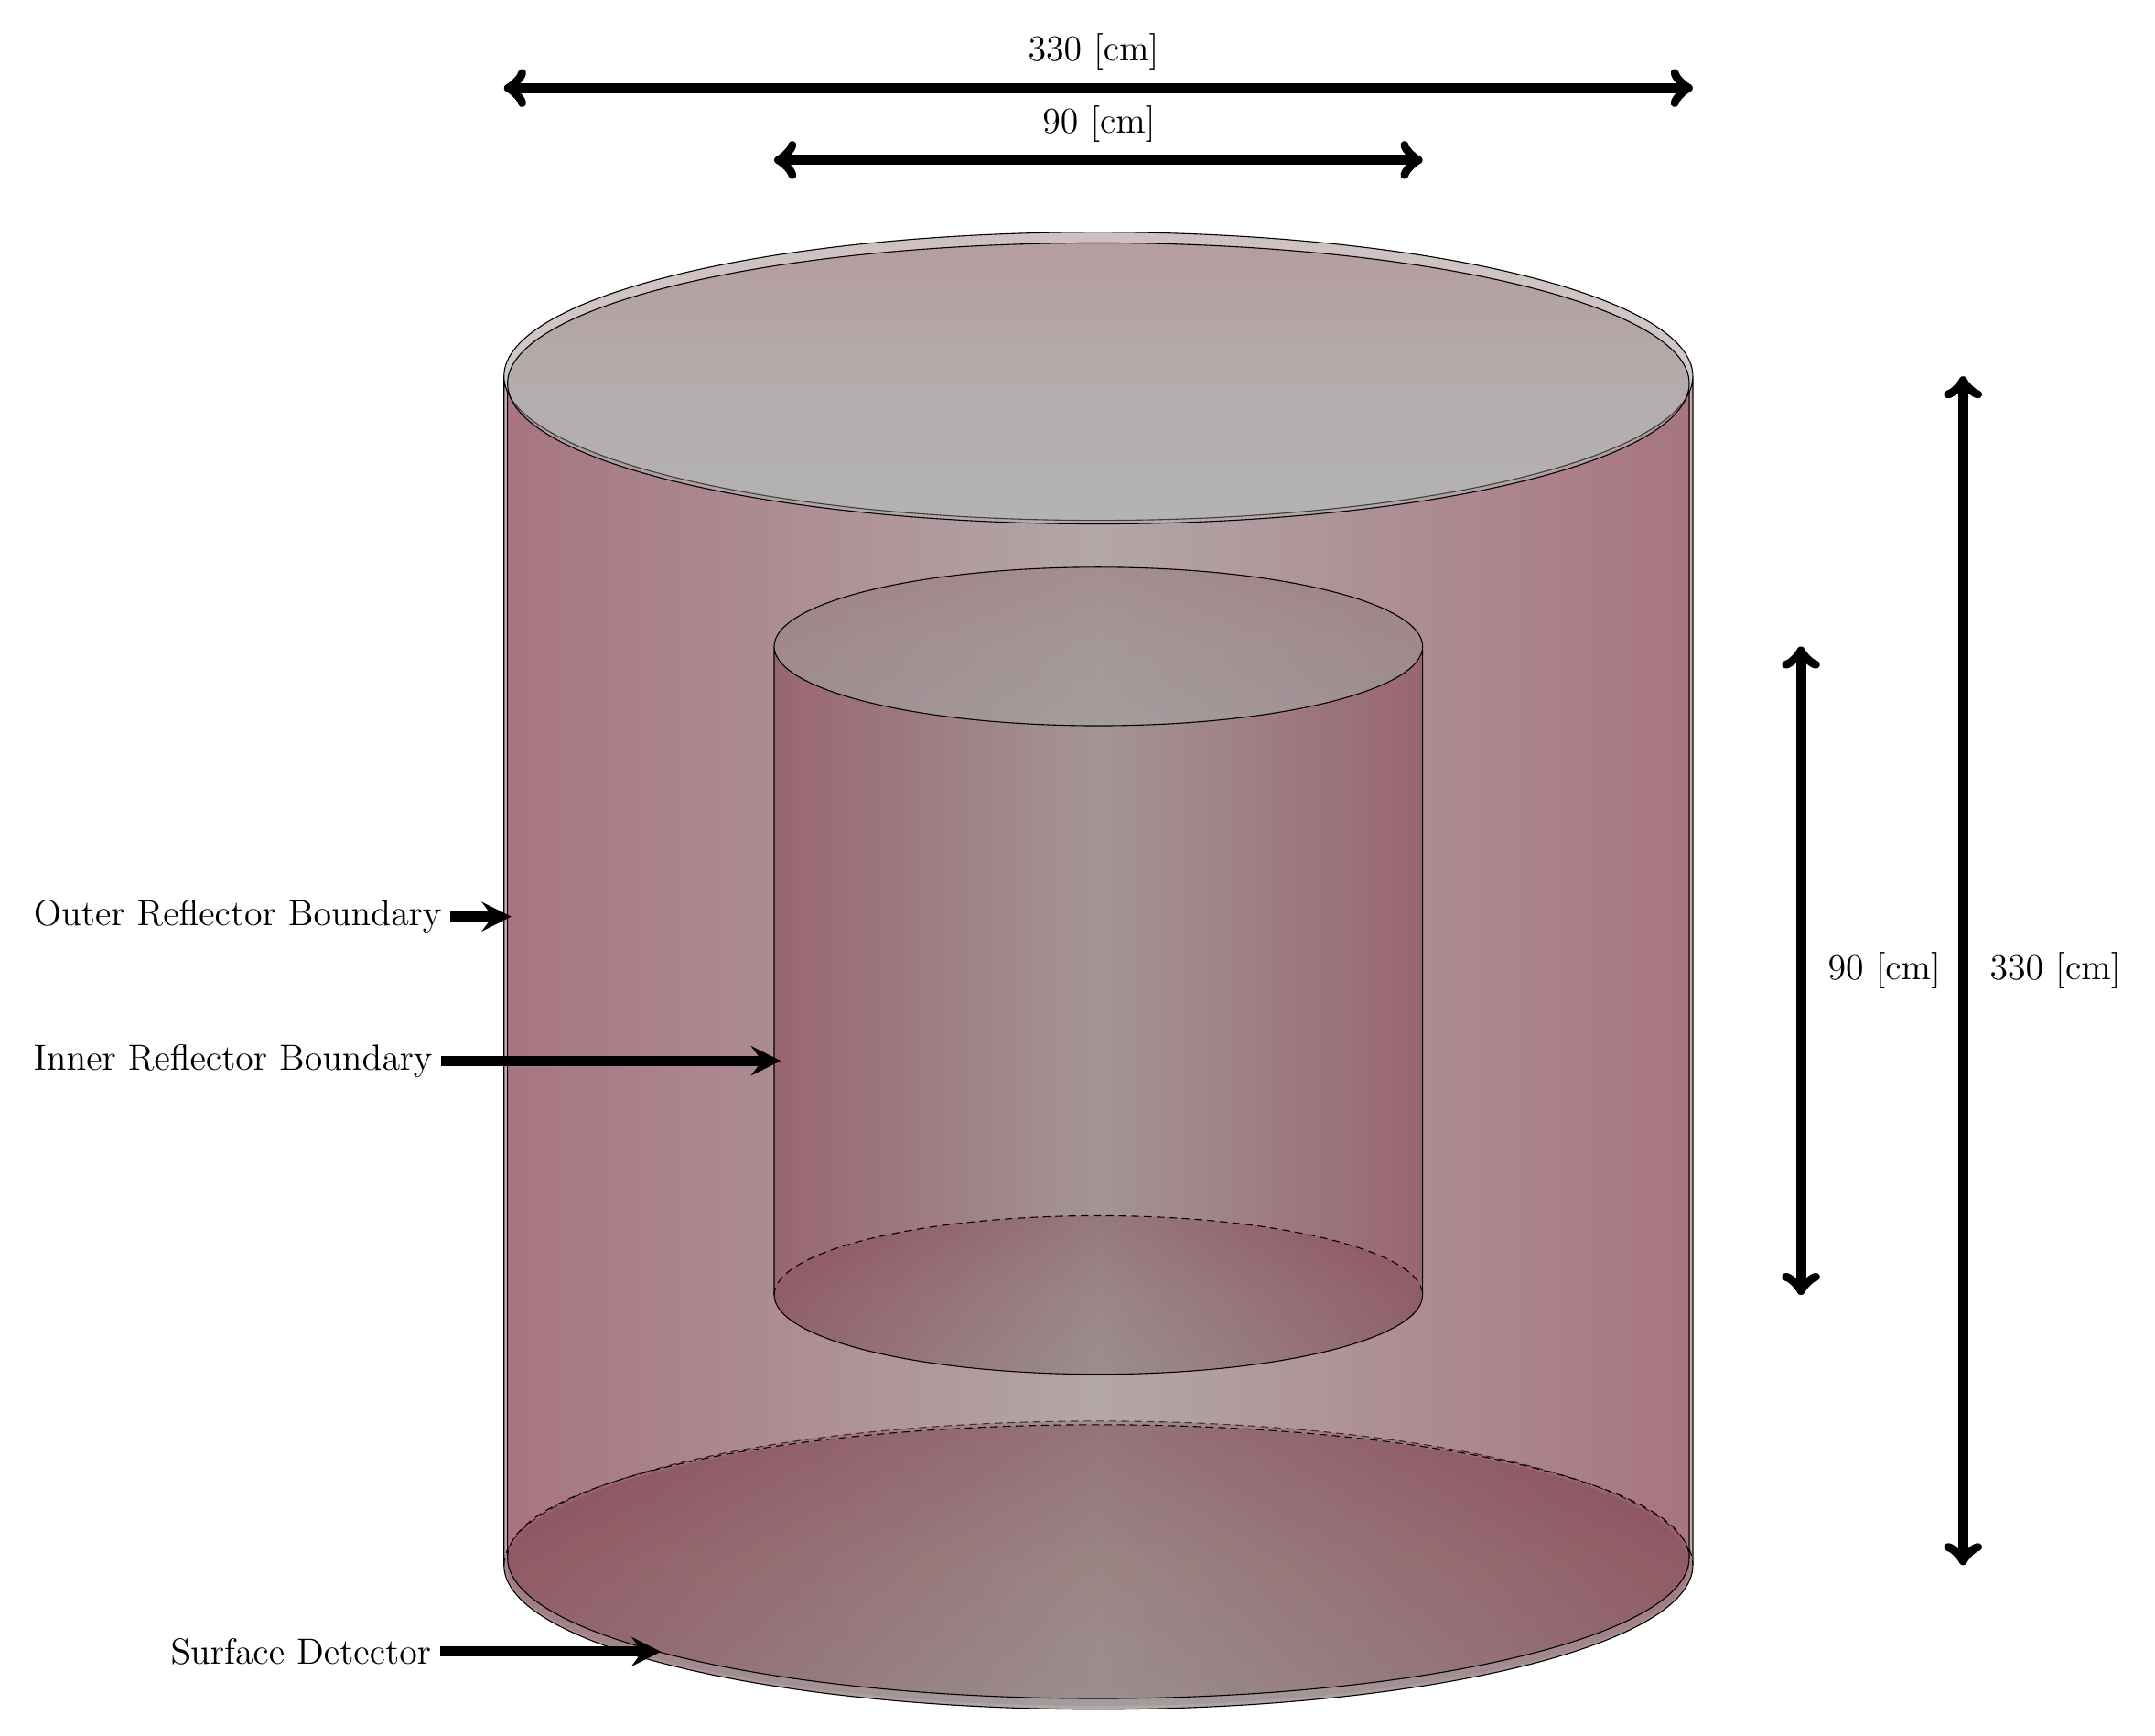
\begin{tikzpicture}
\fill[top color=pink!50!purple,bottom color=pink!10,middle color=pink,shading=axis,opacity=0.25] (0,0) circle (8.25cm and 2.0cm);
\fill[left color=pink!50!purple,right color=pink!50!purple,middle color=pink!50,shading=axis,opacity=0.25] (8.25,0) -- (8.25,16.5) arc (360:180:8.25cm and 2.0cm) -- (-8.25,0) arc (180:360:8.25cm and 2.0cm);
\fill[top color=pink!90!,bottom color=pink!2,middle color=pink!30,shading=axis,opacity=0.25] (0,16.5) circle (8.25cm and 2.0cm);
\draw (-8.25,16.5) -- (-8.25,0) arc (180:360:8.25cm and 2.0cm) -- (8.25,16.5) ++ (-8.25,0) circle (8.25cm and 2.0cm);
\draw[densely dashed] (-8.25,0) arc (180:0:8.25cm and 2.0cm);

\fill[top color=pink!50!purple,bottom color=pink!10,middle color=pink,shading=axis,opacity=0.25] (0,0.0) circle (8.2cm and 1.95cm);
\fill[left color=pink!50!purple,right color=pink!50!purple,middle color=pink!50,shading=axis,opacity=0.25] (8.2,0.1) -- (8.2,16.4) arc (360:180:8.2cm and 1.95cm) -- (-8.2,0.1) arc (180:360:8.2cm and 1.95cm);
\fill[top color=pink!90!,bottom color=pink!2,middle color=pink!30,shading=axis,opacity=0.25] (0,16.4) circle (8.2cm and 1.95cm);
\draw (-8.2,16.3) -- (-8.2,0.1) arc (180:360:8.2cm and 1.95cm) -- (8.2,16.3) ++ (-8.2,0.1) circle (8.2cm and 1.95cm);
\draw[densely dashed] (-8.2,0.1) arc (180:0:8.2cm and 1.85cm);

\fill[top color=pink!50!purple,bottom color=pink!10,middle color=pink,shading=axis,opacity=0.25] (0,3.75) circle (4.5cm and 1.1cm);
\fill[left color=pink!50!purple,right color=pink!50!purple,middle color=pink!50,shading=axis,opacity=0.25] (4.5,3.75) -- (4.5,12.75) arc (360:180:4.5cm and 1.1cm) -- (-4.5,3.75) arc (180:360:4.5cm and 1.1cm);
\fill[top color=pink!90!,bottom color=pink!2,middle color=pink!30,shading=axis,opacity=0.25] (0,12.75) circle (4.5cm and 1.1cm);
\draw (-4.5,12.75) -- (-4.5,3.75) arc (180:360:4.5cm and 1.1cm) -- (4.5,12.75) ++ (-4.5,3.75) (0,12.75) circle (4.5cm and 1.1cm);
\draw[densely dashed] (-4.5,3.75) arc (180:0:4.5cm and 1.1cm);

\node [anchor=west] (out-ref) at (-14.9, 9) {\Large Outer Reflector Boundary};
\node [anchor=west] (in-ref) at (-14.9, 7) {\Large Inner Reflector Boundary};
\node [anchor=west] (det) at (-13, -1.2) {\Large Surface Detector};

\draw [-stealth, line width=4pt, black] (out-ref) -- ++(3.8,0);
\draw [-stealth, line width=4pt, black] (in-ref) -- ++(7.6,0);
\draw [-stealth, line width=4pt, black] (det) -- ++(5.0,0);

\draw [-stealth, <->, line width=4pt, black] ++(-8.25,20.5) -- ++(16.5,0);
\draw [-stealth, <->, line width=4pt, black] ++(12,0) -- ++(0,16.5);

\node [anchor=west] (out-h) at (12.25, 8.25) {\Large 330 [cm]};
\node [anchor=west] (out-d) at (-1.1, 21.0) {\Large 330 [cm]};

\draw [-stealth, <->, line width=4pt, black] ++(-4.5,19.5) -- ++(9,0);
\draw [-stealth, <->, line width=4pt, black] ++(9.75,3.75) -- ++(0,9.0);

\node [anchor=west] (in-h) at (10.0, 8.25) {\Large 90 [cm]};
\node [anchor=west] (in-d) at (-0.9, 20.0) {\Large 90 [cm]};

\end{tikzpicture}
 }%
\caption{Detector Placement Inside Reflector in Sangamon200 and Sangamon20}
\label{fig:det-place}

\end{figure}


This detector measures the outward neutron current (*** serpent outputs units of [number/s], is current still the best word? ***) in $[\frac{\#}{s}]$.  To arrive at the unit of $[\frac{\#}{cm^2s}]$ most are familiar with, the reported outward current is divided by the detector's surface area thusly:
\begin{equation}
J^+ [\frac{\#}{cm^2s}] = \frac{J^+ [\frac{\#}{s}]}{S_{det}[cm^2]}
\end{equation}

After accounting for the surface area, the outward current at the detector is 7.351e+11.

\section{Sangamon1}

Sangamon1 is a 20 MWth helium-cooled pebble bed reactor, fueled with 19.75\% enriched uranium oxycarbide.  While the capacity of Sangamon1 is 10\% that of Sangamon0, it is not possible to simply scale Sangamon0's dimensions down to 90\%.

\subsection{Inner Core Volume Determination}

The first assumption made in the scale-down is that Sangamon0 and Sangamon1 have the same power density, or $\frac{\text{kW}}{\text{g fuel}}$ (*** I called this "power density" as that is how serpent refers to this value.  But, given that it is per unit mass, is "specific power" a better term?***).

It is simple enough to calculate the mass of fuel in Sangamon0:

\begin{equation}
M_{fuel,0} = \frac{4}{3}\pi r_{uco}^3 \rho_{uco} n_{TRISO} n_{pebbles,0}
\end{equation}

Where
\begin{itemize}
\item $M_{fuel}$ is the mass of fuel in Sangamon0,
\item $r_{uco}$ is the radius of the UCO kernel inside a TRISO particle,
\item $\rho_{uco}$ is the density of UCO in $[\frac{g}{cc}]$
\item $n_{TRISO}$ is the number of TRISO particles in one pebble, and
\item $n_{pebbles}$ is the number of pebbles in Sangamon0.
\end{itemize}

Using the parameters in \ref{table:params1}, the power density of Sangamon0 and Sangamon1 is 0.11 $[\frac{kW}{g}]$.  With a power capacity of 20 MWth, one can calculate the total mass of UCO in Sangamon1 as
\begin{equation}
M_{fuel,1} = \frac{20*10^3 [kW]}{0.11[\frac{kW}{g}]} = 181818.18 [g]
\end{equation}
The mass of fuel in a single pebble can be found using the density of UCO and the total volume of UCO kernels in a single pebble, as above.  The number of pebbles in the entire reactor, then, is found by dividing the total mass of fuel by the mass of fuel in one pebble, as follows:

\begin{equation}
n_{pebbles,1} = \frac{M_{fuel,1}}{\frac{4}{3}r_{uco}^3n_{TRISO}\rho_{uco}}
\end{equation}

Rounding up, as it is not possible to have a partial pebble, we arrive at the value in \ref{table:params1}.

Knowing the number of pebbles is not enough - the exact dimensions of the active core region are still undefined.  To determine the volume of this space, the concept of the packing fraction - the ratio of the volume of objects (the pebbles) to the total volume of their container (the active core) - can be used.  The packing of even uniform objects in a 3-dimensional space is a complicated problem, often analyzed in the context of material studies or grain silos \cite{tulluri_analysis_nodate}.  For this reactor, it is assumed the pebble behavior can be described as random loose packing \cite{tulluri_analysis_nodate} - the pebbles have entered the core and fallen in an asystematic manner and have not been shaken to pack them in a more optimal fashion.  Such packing generally has a packing fraction in the range of 0.56 to 0.60 \cite{tulluri_analysis_nodate}.  Using the definition of the packing fraction, and previously defined terms, the active core volume is

\begin{equation}
V_{core,1} = \frac{ n_{pebbles,1}\frac{4}{3}\pi r_{pebble}^3 }{ \phi }
\end{equation}

Using the formula for the volume of a cylinder, one can plot possible values of $r_{core,1}$ and $h_{core,1}$ that satisfy the volume requirement.

\begin{figure}[h!]
\centering
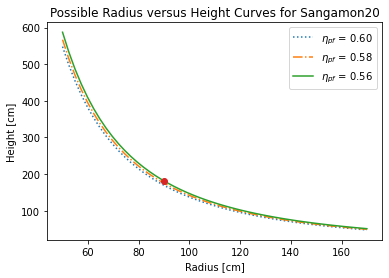
\includegraphics[width = 10cm]{figures/act-core-RH.png}
\caption{Curve of Possible Height and Radii by Packing Fraction}
\label{fig:rh-vol}
\end{figure}

It is also true that the most critical configurations for a cylinder are either a "fat" shape, where the height is equal to the diameter, or a flat "pancake" shape, that height is much less than diameter.  As a very flat shape is not very convienient for a reactor, the former is chosen.  The point indicated in \ref{fig:rh-vol} shows the radius and height selected for Sangamon1 - a radius of 90 cm, and a height of 180 cm.

\subsection{Graphite Reflector Thickness Determination}

The reflector must be sufficiently thick to keep the reactor critical, and protect the pressure vessel.  To ensure this, the outward current must be less than or equal to the outward current in Sangamon0 at the outer reflector boundary.  The detector layout in Sangamon1 is identical to \ref{fig:det-place}.

\section{Fuel Composition}

The isotopic composition of the pebbles is based on the number of passes the pebble has theoretically experienced.  There are seven possible pebble compositions, one for each of the six 6-month passes, plus an additional composition for fresh pebbles.  The seven pebble compositions are represented equally in number in the core, and the "kinds" of pebbles are randomly distributed throughout the core.

The exact isotopic composition is approximated by running a burnup calculation using Serpent2 for a single pebble in a unit square.  It uses a reflective boundary condition to simulate the presence of other pebbles or the reflector.  The void in the square is filled with helium.  While the full-core models homogenize the pebbles, the TRISO particles in the single pebble burnup models are individually modeled.  Just as with the location of the pebbles in the full core, the Serpent2 particle dispersal routine generated the TRISO particle locations.

\begin{figure}[H]
\centering
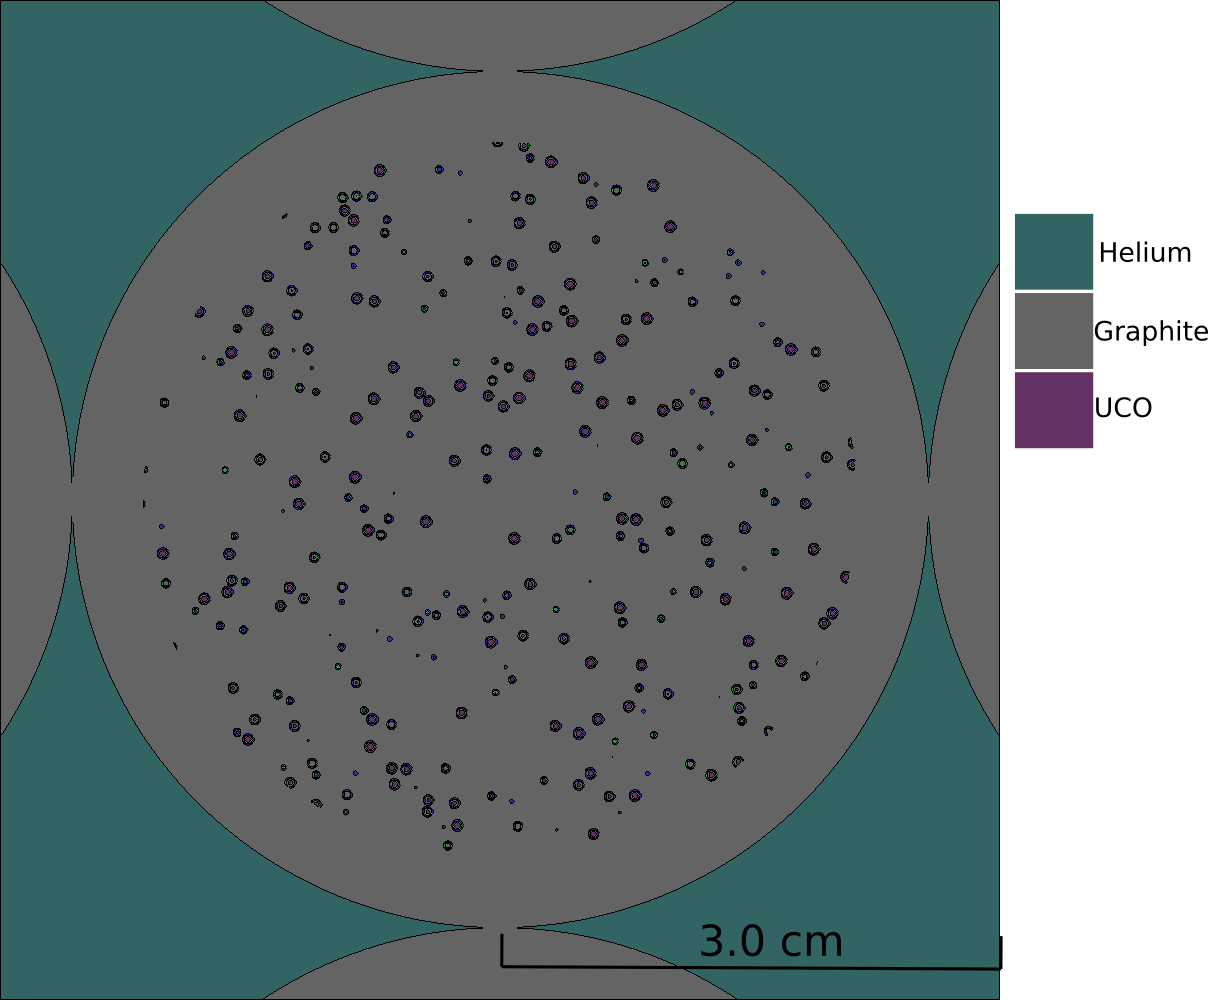
\includegraphics[width = 10cm]{figures/burn-20.png}
\caption{Geometry of the Single-Pebble Burnup Calculation for Sangamon20}
\label{fig:burn-20}
\end{figure}

Once the isotopic compositions are determined, the pebbles are homogenized by volume, to improve performance.  The volume of a TRISO particle, and more specifically, a UCO kernel, is assumed constant.

\section{Reactor Sensitivity to Pebble Locations and Symmetry}

As the pebble locations and compositions are determined randomly, it is entirely possible to have "bands" in the reactor where multiple pebbles of same (or similar) burnup form lines or pockets.  In the interest of better characterizing the neutronics of the reactor, a sensitivity analysis tested different pebble compositon locations.  The "shuffling" test maintained the pebble locations, but changed what composition the individual pebbles were.  A second test analyzed the effects of utilizing a symmetry simplification, in order to improve computational speed.  The core was modeled using a $\frac{1}{6}$ slice.  For 6 tests, the area the representative slice was taken from changed as shown in \ref{fig:slicetest}.  In each test, all other parameters remain the same.

\begin{figure}[h!]
\centering

\includegraphics[width=0.6\linewidth]{figures/run-layout.png}
\caption{Symmetry Test Run Layouts}
\label{fig:slicetest}
\end{figure}